\ProvidesFile{seminar9.tex}

\section{Семинар 9}

Для удобства независимое множество иногда называется анти-кликой.

\subsection{Задача 1}

Докажите, что для всех возможных значений переменных верно: $R(s,t) = R(t,s), \\
R(1,n) = 1, R(2,n) = n, R(3,3) = 6$.

\begin{proof}
Свойство $R(s,t) = R(t,s)$ очевидно из определения (надо поменять синий и красный цвет).

$R(1,n) = 1$ тоже ясно. Существует один неизоморфный граф на 1 вершине, для которого всё очевидно.

$R(2,n) = n$ уже стоит пояснить. Рассмотрим граф на $n$ вершинах. Ясно, что либо есть пара знакомых людей, либо никто никого не знает. Поэтому $R(2,n) \leq n$.

Предположим, что $R(2,n) = s < n$. Если в графе на $s$ вершинах нет ребра, то ясно, что нет ни клики на 2 вершинах, ни анти-клики на $n$ вершинах (так как банально $s < n$).

$R(3, 3) = 6$. То, что $R(3, 3) \leq 6$ -- ясно из рассуждения на 8 красном задаче.

То, что $R(3, 3)$ в точности равно 6 доказывается с помощью контр-примера на 5. Важно, что контр-пример на 5 автоматически доказывает, что меньше 5 тем более не получится (ну так как можно выкинуть вершины из графа на 5 вершинах и рассуждения останутся верны).
\end{proof}

\subsection{Задача 2}

Докажите, что: $\displaystyle R(s, t) \leq C^{t-1}_{s+t-2}$

\begin{proof}
Будем доказывать по индукции. 

Ясно, что $R(2,n) = n = C^{2-1}_{n+2-2}$

Отсюда видно, что наша оценка в некотором смысле точная (то есть хоть где-то она достигается).

Воспользуемся теоремой Рамсея и предположением индукции:
\[
R(s, t) \leq \underbrace{R(s-1,t)}_{\leq C^{t-1}_{s+t-3}} + \underbrace{R(s, t-1)}_{\leq C^{t-2}_{s+t-3}} \leq C^{t-1}_{s+t-2} \quad (C^k_n = C^k_{n-1} + C^{k-1}_{n-1})
\]
\end{proof}

\subsection{Задача 3}

Докажите, что $R(3,4) = 9$.

\begin{proof}
    $R(3,4) \leq \underbrace{R(2, 4)}_{4} + \underbrace{R(3, 3)}_{6} - 1 = 9$ в силу усиления теоремы Рамсея. 

    Контр-пример на 8 вот:

    \begin{figure}[H]
        \centering
        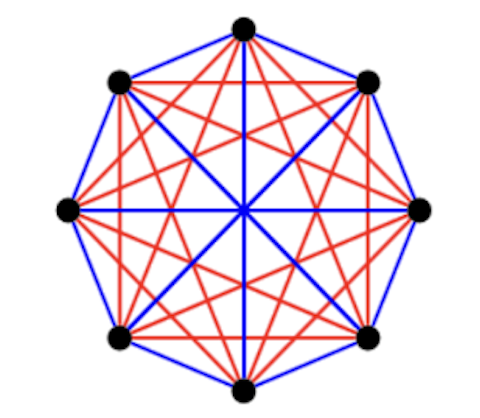
\includegraphics[width=0.25\linewidth]{sem9_task3.png}
    \end{figure}
\end{proof}

\subsection{Задача 4}

Докажите, что $R(3,5) = 14$.

\begin{proof}
    $R(3,5) \leq \underbrace{R(2, 5)}_{5} + \underbrace{R(3, 4)}_{9} = 14$

    Контр-пример на 13 строится довольно интересно, с рассмотрением некоторых специфичных остатков из группы $\mathbb{Z}_{13}$. Можно почитать \href{https://math.stackexchange.com/questions/190982/prove-ramsey-number-r3-5-14}{тут}
\end{proof}


\subsection{Задача 5}

Докажите, что $R(4, 4) = 18$

\begin{proof}
    $R(4, 4) \leq \underbrace{R(3, 4)}_{9} + \underbrace{R(4, 3)}_{9} = 18$

    Контр-пример на 17 \href{https://www.cut-the-knot.org/arithmetic/combinatorics/Ramsey44.shtml}{тут}
\end{proof}

Если вам любопытно, то вот что известно человечеству о числах Рамсея:

\begin{figure}[H]
    \centering
    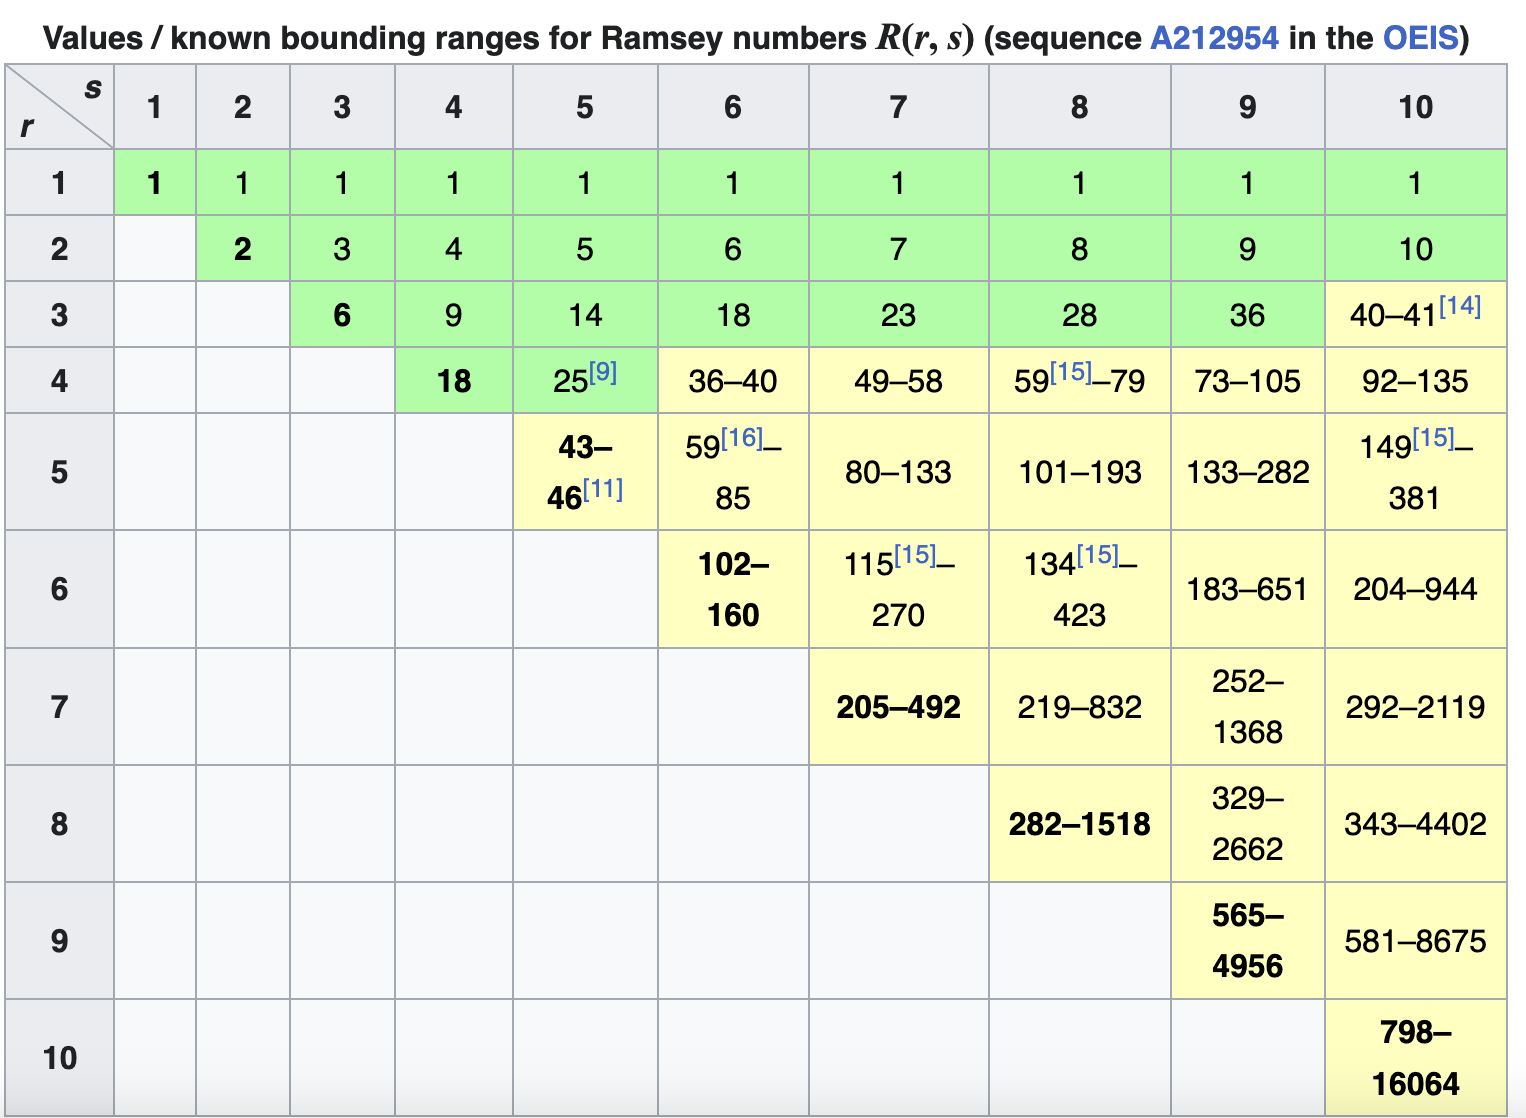
\includegraphics[width=0.75\linewidth]{sem09_known_ramsey_numbers.png}
\end{figure}

\subsection{Задача 6}

\begin{proof}
    Доказательство аналогично доказательству теоремы Рамсея. 

    
\end{proof}